\documentclass{article}
\usepackage[paperwidth=15.35in,paperheight=6.7in,margin=0.14in]{geometry}
\usepackage{amsmath}
\usepackage{tikz}
\usetikzlibrary{arrows.meta,positioning,calc}
\pagestyle{empty}

\begin{document}
\noindent
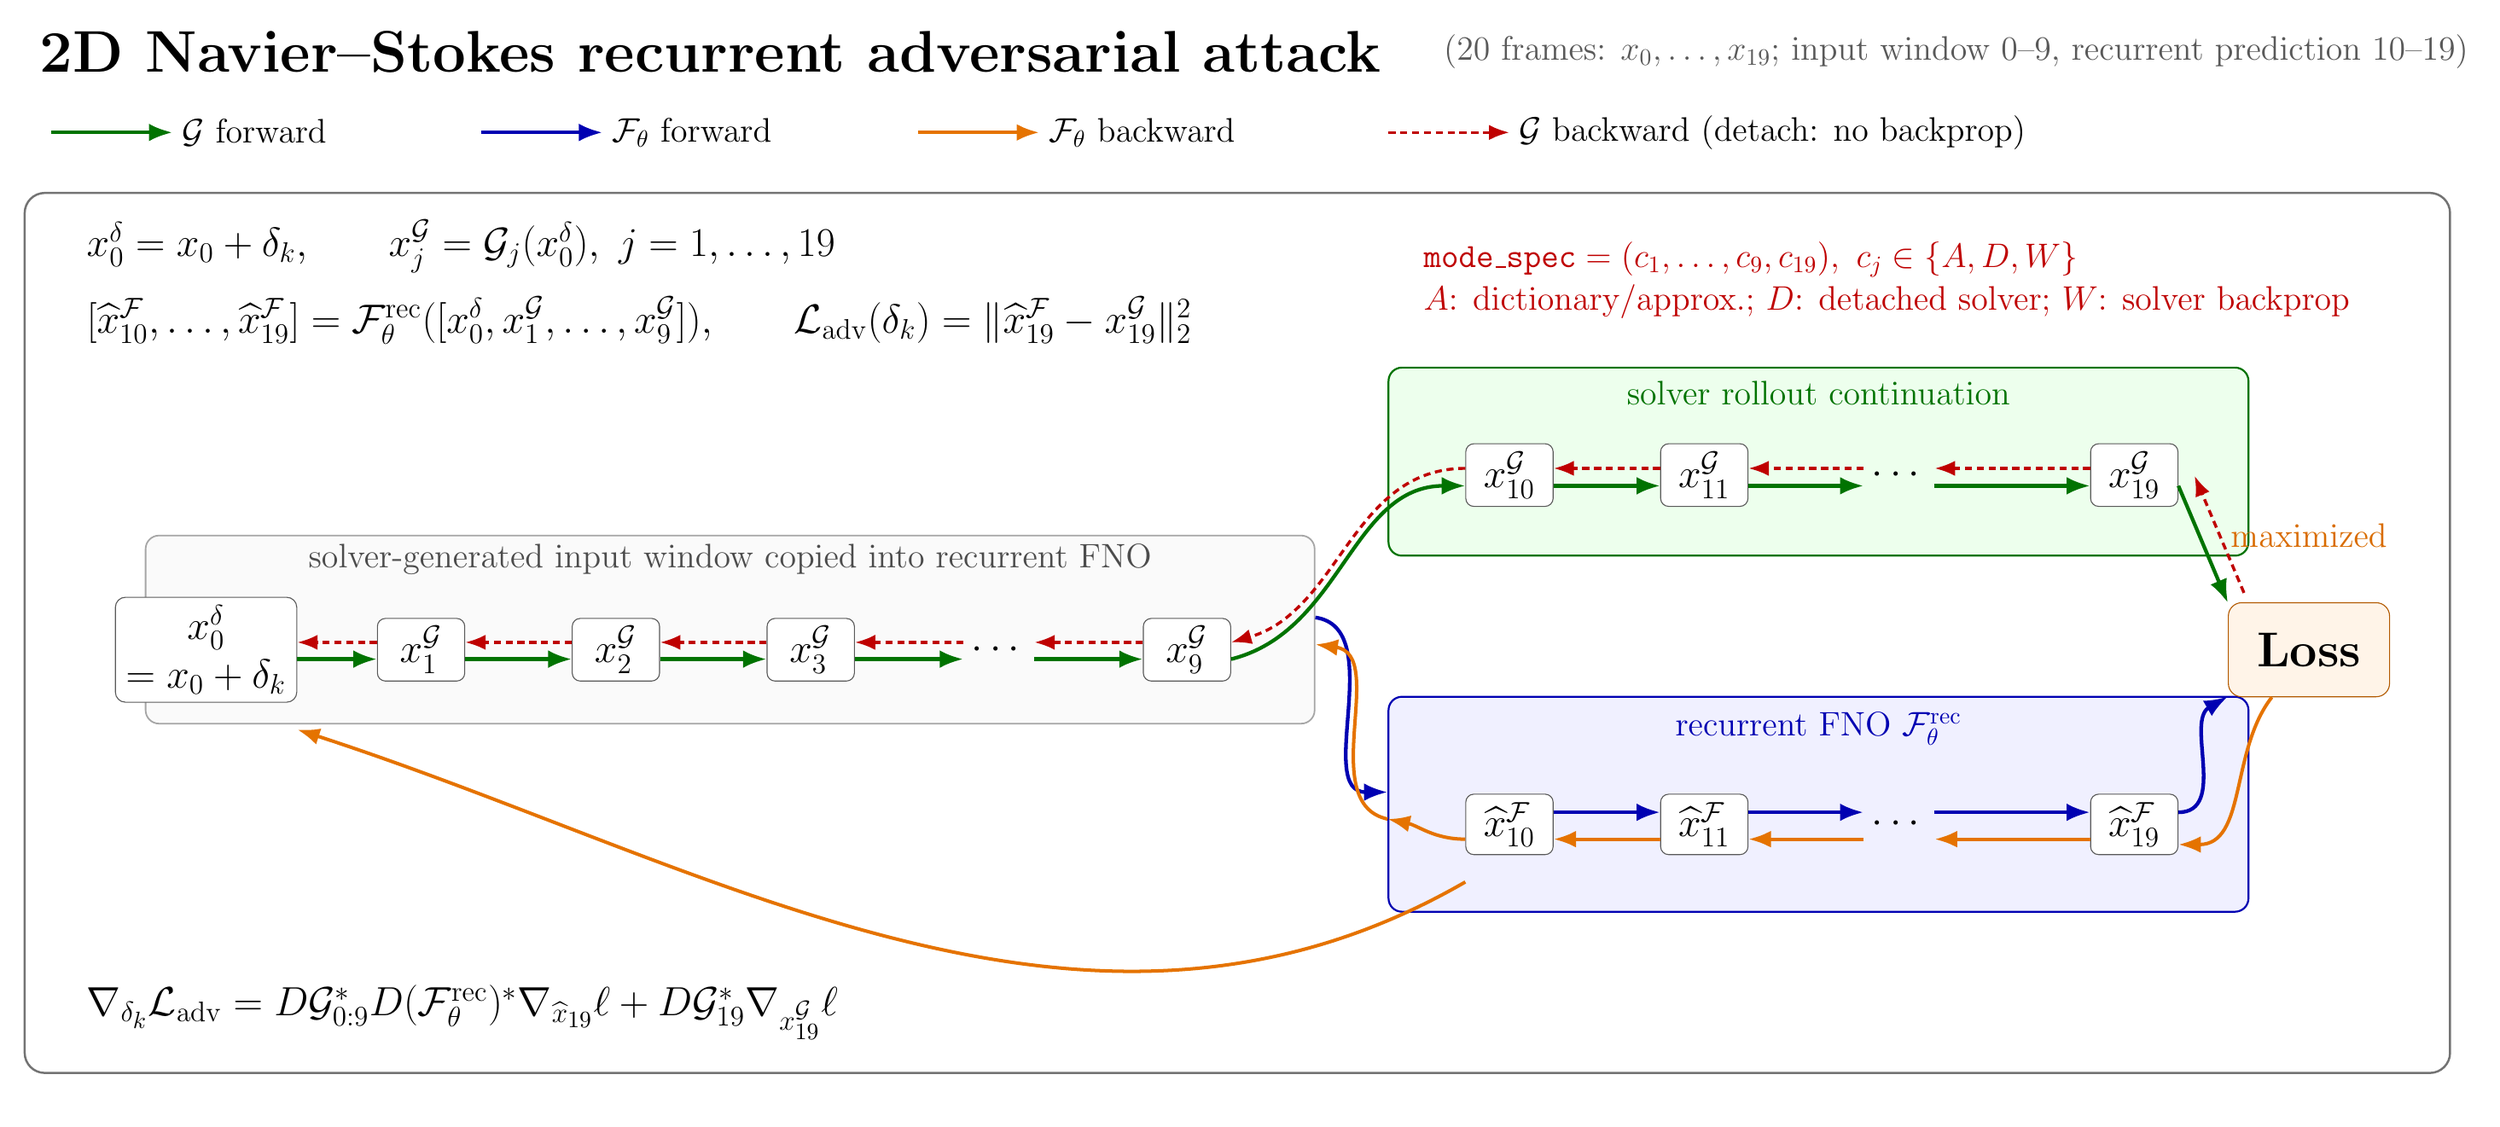
\begin{tikzpicture}[
  x=1mm,y=1mm,
  >=Latex,
  font=\sffamily,
  panel/.style={draw=black!55, rounded corners=3mm, line width=0.9pt, fill=white},
  band/.style={draw=black!35, rounded corners=2mm, line width=0.65pt, fill=black!2},
  frame/.style={draw=black!65, rounded corners=1.2mm, fill=white, minimum width=13mm, minimum height=9mm, align=center, font=\LARGE\bfseries},
  input/.style={draw=black!65, rounded corners=1.5mm, fill=white, minimum width=27mm, minimum height=12mm, align=center, font=\LARGE},
  solverband/.style={draw=green!45!black, rounded corners=2mm, fill=green!7, line width=0.8pt},
  modelband/.style={draw=blue!70!black, rounded corners=2mm, fill=blue!6, line width=0.8pt},
  loss/.style={draw=orange!70!black, rounded corners=2mm, fill=orange!9, minimum width=24mm, minimum height=14mm, align=center, font=\huge\bfseries},
  formula/.style={font=\LARGE, anchor=west, align=left},
  backformula/.style={font=\LARGE, anchor=west, align=left},
  smallnote/.style={font=\Large, text=black!65, align=center},
  fsolver/.style={->, draw=green!45!black, line width=1.55pt},
  fmodel/.style={->, draw=blue!70!black, line width=1.55pt},
  bmodel/.style={->, draw=orange!90!black, line width=1.45pt},
  bsolver/.style={->, draw=red!75!black, line width=1.25pt, densely dashed}
]

% Title and legend
\node[font=\Huge\bfseries, anchor=west] at (5,160) {2D Navier--Stokes recurrent adversarial attack};
\node[font=\Large, anchor=west, text=black!65] at (214,160) {(20 frames: $x_0,\ldots,x_{19}$; input window 0--9, recurrent prediction 10--19)};
\draw[fsolver] (8,148) -- ++(18,0) node[right, black, font=\Large] {$\mathcal G$ forward};
\draw[fmodel] (72,148) -- ++(18,0) node[right, black, font=\Large] {$\mathcal F_\theta$ forward};
\draw[bmodel] (137,148) -- ++(18,0) node[right, black, font=\Large] {$\mathcal F_\theta$ backward};
\draw[bsolver] (207,148) -- ++(18,0) node[right, black, font=\Large] {$\mathcal G$ backward (detach: no backprop)};

% Main panel
\draw[panel] (4,8) rectangle (365,139);

\node[formula] at (12,131)
  {$x_0^\delta=x_0+\delta_k,\qquad
    x_j^{\mathcal G}=\mathcal G_j(x_0^\delta),\ j=1,\ldots,19$};
\node[formula] at (12,120)
  {$[\widehat{x}_{10}^{\mathcal F},\ldots,\widehat{x}_{19}^{\mathcal F}]
    =\mathcal F_\theta^{\mathrm{rec}}([x_0^\delta,x_1^{\mathcal G},\ldots,x_9^{\mathcal G}]),
    \qquad
    \mathcal L_{\mathrm{adv}}(\delta_k)=
    \|\widehat{x}_{19}^{\mathcal F}-x_{19}^{\mathcal G}\|_2^2$};
\node[backformula] at (12,17)
  {$\nabla_{\delta_k}\mathcal L_{\mathrm{adv}}
    =
    D\mathcal G_{0:9}^{*}D(\mathcal F_\theta^{\mathrm{rec}})^{*}\nabla_{\widehat{x}_{19}}\ell
    +
    D\mathcal G_{19}^{*}\nabla_{x_{19}^{\mathcal G}}\ell$};

% Shared input window: x0..x9, one row only.
\node[band, minimum width=174mm, minimum height=28mm] (inputband) at (109,74) {};
\node[smallnote, text=black!70] at (109,84.5) {solver-generated input window copied into recurrent FNO};
\node[input] (x0) at (31,71) {$x_0^\delta$\\[-0.5mm]$=x_0+\delta_k$};
\node[frame] (g1) at (63,71) {$x_1^{\mathcal G}$};
\node[frame] (g2) at (92,71) {$x_2^{\mathcal G}$};
\node[frame] (g3) at (121,71) {$x_3^{\mathcal G}$};
\node[font=\LARGE] (gd1) at (149,71) {$\cdots$};
\node[frame] (g9) at (177,71) {$x_9^{\mathcal G}$};

% Solver truth from x10..x19.
\node[solverband, minimum width=128mm, minimum height=28mm] (solverout) at (271,99) {};
\node[smallnote, text=green!45!black] at (271,109.2) {solver rollout continuation};
\node[frame] (g10) at (225,97) {$x_{10}^{\mathcal G}$};
\node[frame] (g11) at (254,97) {$x_{11}^{\mathcal G}$};
\node[font=\LARGE] (gd2) at (283,97) {$\cdots$};
\node[frame] (g19) at (318,97) {$x_{19}^{\mathcal G}$};

% Recurrent FNO prediction from x10..x19.
\node[modelband, minimum width=128mm, minimum height=32mm] (modelout) at (271,48) {};
\node[smallnote, text=blue!70!black] at (271,59.2) {recurrent FNO $\mathcal F_\theta^{\mathrm{rec}}$};
\node[frame] (f10) at (225,45) {$\widehat{x}_{10}^{\mathcal F}$};
\node[frame] (f11) at (254,45) {$\widehat{x}_{11}^{\mathcal F}$};
\node[font=\LARGE] (fd2) at (283,45) {$\cdots$};
\node[frame] (f19) at (318,45) {$\widehat{x}_{19}^{\mathcal F}$};

% Loss
\node[loss] (loss) at (344,71) {Loss};
\node[smallnote, text=orange!85!black] at (344,88) {maximized};

% Forward: solver produces all ground-truth frames; only x10--x19 are shown as the comparison branch.
\draw[fsolver] ([yshift=-1.4mm]x0.east) -- ([yshift=-1.4mm]g1.west);
\draw[fsolver] ([yshift=-1.4mm]g1.east) -- ([yshift=-1.4mm]g2.west);
\draw[fsolver] ([yshift=-1.4mm]g2.east) -- ([yshift=-1.4mm]g3.west);
\draw[fsolver] ([yshift=-1.4mm]g3.east) -- ([yshift=-1.4mm]gd1.west);
\draw[fsolver] ([yshift=-1.4mm]gd1.east) -- ([yshift=-1.4mm]g9.west);
\draw[fsolver] ([yshift=-1.4mm]g9.east) to[out=14,in=180] ([yshift=-1.6mm]g10.west);
\draw[fsolver] ([yshift=-1.6mm]g10.east) -- ([yshift=-1.6mm]g11.west);
\draw[fsolver] ([yshift=-1.6mm]g11.east) -- ([yshift=-1.6mm]gd2.west);
\draw[fsolver] ([yshift=-1.6mm]gd2.east) -- ([yshift=-1.6mm]g19.west);
\draw[fsolver] ([yshift=-1.6mm]g19.east) -- (loss.150);

% Forward: the copied window enters the recurrent FNO, which predicts x10--x19.
\draw[fmodel] ([yshift=1.8mm]inputband.east) to[out=-8,in=180] ([yshift=1.8mm]modelout.west);
\draw[fmodel] ([yshift=1.8mm]f10.east) -- ([yshift=1.8mm]f11.west);
\draw[fmodel] ([yshift=1.8mm]f11.east) -- ([yshift=1.8mm]fd2.west);
\draw[fmodel] ([yshift=1.8mm]fd2.east) -- ([yshift=1.8mm]f19.west);
\draw[fmodel] ([yshift=1.8mm]f19.east) to[out=0,in=210] (loss.210);

% Backward through the recurrent FNO branch, drawn step by step rather than as one long jump.
\draw[bmodel] (loss.232)
  to[out=232,in=0] ([yshift=-3.0mm]f19.east);
\draw[bmodel] ([yshift=-2.2mm]f19.west) -- ([yshift=-2.2mm]fd2.east);
\draw[bmodel] ([yshift=-2.2mm]fd2.west) -- ([yshift=-2.2mm]f11.east);
\draw[bmodel] ([yshift=-2.2mm]f11.west) -- ([yshift=-2.2mm]f10.east);
\draw[bmodel] ([yshift=-2.2mm]f10.west)
  to[out=180,in=-12] ([yshift=-2.2mm]modelout.west);
\draw[bmodel] ([yshift=-2.2mm]modelout.west)
  to[out=168,in=-8] ([yshift=-2.2mm]inputband.east);
\draw[bmodel] ([yshift=-4.0mm]f10.south west)
  to[out=210,in=-18,looseness=0.95] ([yshift=-4.0mm]x0.south east);

% Solver backward branch. Red dashed arrows run parallel to the green solver path.
\draw[bsolver] ([xshift=2.4mm,yshift=1.5mm]loss.150)
  -- ([xshift=2.4mm,yshift=-0.1mm]g19.east);
\draw[bsolver] ([yshift=1.0mm]g19.west) -- ([yshift=1.0mm]gd2.east);
\draw[bsolver] ([yshift=1.0mm]gd2.west) -- ([yshift=1.0mm]g11.east);
\draw[bsolver] ([yshift=1.0mm]g11.west) -- ([yshift=1.0mm]g10.east);
\draw[bsolver] ([yshift=1.0mm]g10.west)
  to[out=180,in=16] ([yshift=1.1mm]g9.east);
\draw[bsolver] ([yshift=1.1mm]g9.west) -- ([yshift=1.1mm]gd1.east);
\draw[bsolver] ([yshift=1.1mm]gd1.west) -- ([yshift=1.1mm]g3.east);
\draw[bsolver] ([yshift=1.1mm]g3.west) -- ([yshift=1.1mm]g2.east);
\draw[bsolver] ([yshift=1.1mm]g2.west) -- ([yshift=1.1mm]g1.east);
\draw[bsolver] ([yshift=1.1mm]g1.west) -- ([yshift=1.1mm]x0.east);
\node[smallnote, text=red!75!black, anchor=west, align=left] at (211,126)
  {$\texttt{mode\_spec}=(c_1,\ldots,c_9,c_{19}),\ c_j\in\{A,D,W\}$\\
   $A$: dictionary/approx.; $D$: detached solver; $W$: solver backprop};

\end{tikzpicture}
\end{document}
